\documentclass[fr]{../../../../../../eplexam}
\usepackage{../../../../../../eplchem}
\usepackage{../../../../../../eplunits}

\hypertitle{Chimie et chimie physique}{3}{FSAB}{1302}{2017}{Janvier}{All}
{Martin Braquet}
{Hervé Jeanmart et Joris Proost}

\section{Théorie (thermodynamique)}

On considère un gaz parfait diatomique qui s'étend de manière adiabatique irréversible contre une pression externe constante.
\begin{enumerate}
  \item Comment varie l'entropie lors de cette expansion?
  \item Enoncez le second principe de la thermodynamique.
  \item Sur base du second principe, justifier votre réponse au point 1.
  \item Le gaz passe de la température $T_1$ à $T_2$ lors de la transformation, calculer $T_2$ en fonction de $T_1$, $p_i$ (pression interne) et $p_e$ (pression externe).
  \item Comment $T_2$ varie-t-il, par rapport au cas irréversible, si l'expansion était réversible? Justifiez de manière physique et non mathématique.
\end{enumerate}

\begin{solution}

\begin{enumerate}
  \item L'entropie augmente.
  \item Toute transformation d'un système thermodynamique s'effectue avec augmentation de l'entropie globale incluant l'entropie du système et du milieu extérieur.
  $$\Delta S=\Delta S_i+\Delta S_e \ge 0$$
  avec $\Delta S_e=\frac{\delta Q}{T}$ et $\Delta S_i\ge 0$.
  \item Puisque la transformation est adiabatique, $\delta Q=0\Rightarrow \Delta S_i=0$. 
  
  On a donc
  $$\Delta S=\Delta S_e \ge 0,$$
  soit une augmentation de l'entropie totale.
  \item 
  On a dans le cas irréversible
  $$\Delta U=Q+W=W=-\int_1^2p_e\mbox{d}V$$
  $$ C_v(T_2-T_1)=-p_e(V_2-V_1)  \mbox{  (pression externe constante)}$$
  $$ 5/2nR(T_2-T_1)=-p_e(\frac{nRT_2}{p_e}-\frac{nRT_1}{p_i})$$
  $$ 5/2T_2+T_2=p_e\frac{T_1}{p_i}+5/2T_1$$
  $$ \Rightarrow T_2=\frac{2}{7}(\frac{p_e}{p_i}+5/2)T_1$$
  \item La température serait plus basse dans le cas réversible. Dans l'expansion irréversible, des pertes (dues entre autres à l'effet Joule) élèvent la température.
  
  La pression à l'interface dans le cas réversible est plus élevée que la pression atmosphérique.
  $$\Delta U_{\mbox{rév}}=W_{\mbox{rév}}=-\int_1^2p\mbox{d}V<-\int_1^2p_e\mbox{d}V=W_{\mbox{irr}}=\Delta U_{\mbox{irr}}$$
  $$T_{2,\mbox{rév}}-T_1<T_{2,\mbox{irr}}-T_{1}$$
  $$\Rightarrow T_{2,\mbox{rév}}<T_{2,\mbox{irr}}$$
  
\end{enumerate}

\end{solution}

\section{Cycle}

On considère un système fermé parcourant un cycle moteur réversible composé de 5 transformations:
\begin{itemize}
  \item $1 \to 2$: compression adiabatique
  \item $2 \to 3$: échauffement isochore
  \item $3 \to 4$: échauffement isobare
  \item $4 \to 5$: détente adiabatique
  \item $5 \to 1$: refroidissement isochore
\end{itemize}
Le gaz contenu dans le système est de l'air (gaz parfait) dont les propriétés sont constantes et telles que $\gamma=1,3$.
\begin{enumerate}
  \item La chaleur apportée lors des échauffements est de \SI{2000}{\kilo\joule\per\kilogram} et le travail total produit par le cycle est de \SI{1000}{\kilo\joule\per\kilogram} (en valeur absolue). La pression maximale est de 75 bar.
    À partir de ces valeurs, on vous demande de compléter le
    tableau ci-dessous en justifiant succinctement vos résultats.
    \begin{center}
      \begin{tabular}{|c|cccc|}
        \hline
        & $p[\si{\bar}]$ & $v[m^3/kg]$ & $T[\si{\kelvin}]$ & $S-S_1[J/(kg*K)]$\\
        \hline
        1 & 1 &  & 300 & \\
        \hline
        2 &  &  &  & \\
        \hline
        3 &  &  &  & \\
        \hline
        4 &  &  &  & \\
        \hline
        5 &  &  &  & \\
        \hline
      \end{tabular}
    \end{center}
  \item Calculez le rendement de ce cycle.
  
\end{enumerate}
\textbf{Note}: Vous devriez être confronté à une équation implicite pour résoudre ce problème, je vous invite à la résoudre en l'approchant par quelques itérations.

\begin{solution}

Dans certains exercices, il peut être utile de commencer pas la dernière question, c'est possible d'obtenir le rendement dès le début:
$$\eta=\frac{|W_{tot}|}{Q_{HOT}}=\frac{10^6}{2*10^6}=0,5$$
On cherche les capacités calorifiques:
$$ \frac{c_p}{c_v}=\gamma=1,3 \qquad c_p-c_v=R^*$$
$$ \Rightarrow c_p=1243,1 \: [J/kg.K] \qquad c_v=956\: [J/kg.K]$$
On rappelle aussi que $R^*=R/M_m=287,058\:[J/(kg*K)]$.
$$v_5=v_1=\frac{R^*T_1}{p_1}=0,861174\:[m^3/kg]$$
On trouve aussi la ligne 5:
$$Q_{2-3}+Q_{3-4}=2*10^6\:[J/kg]$$
$$W_{tot}=-10^6\:[J/kg]$$
$$0=\Delta U=Q+W=Q_{2-3}+Q_{3-4}+Q_{5-1}+W=2*10^6+Q_{5-1}-10^6$$
$$\Rightarrow Q_{5-1}=\Delta U_{5-1}=-10^6\:(W_{5-1}=0)$$
$$c_v(T_1-T_5)=-10^6\Rightarrow T_5=300+\frac{10^6}{956}=1346K$$
$$p_5=\frac{R^*T_5}{v_5}=4,48675\:[bar]$$
On trouve ensuite la ligne 4 puisque la transformation 4-5 est adiabatique:
$$v_4=v_5(\frac{p_5}{p_4})^{1/\gamma}=0,0986784\:[m^3/kg]$$
$$T_4=\frac{p_4v_4}{R^*}=2578,18K$$
On a ce tableau-ci en complétant avec les données trouvées:
\[
      \begin{tabular}{|c|cccc|}
        \hline
        & $p[\si{\bar}]$ & $v[m^3/kg]$ & $T[\si{\kelvin}]$ & $S-S_1[J/(kg*K)]$\\
        \hline
        1 & 1 & 0,861174 & 300 & 0\\
        \hline
        2 &  &  &  & 0\\
        \hline
        3 & 75 &  &  & \\
        \hline
        4 & 75 & 0,0986784 & 2578,18 & \\
        \hline
        5 & 4,48675 & 0,861174 & 1346 & \\
        \hline
      \end{tabular}
    \]
Il reste à utiliser la donnée avec la chaleur fournie à la source chaude.

On sait que
\begin{itemize}
    \item $Q_{2-3}+Q_{3-4}=2*10^6\:[J/kg]$
    \item $Q_{2-3}=c_v(T_3-T_2)$  (isochore)
    \item $Q_{3-4}=c_p(T_4-T_3)$  (isobare)
    \item $V_2=V_1\bigg(\frac{T_1}{T_2}\bigg)^{\frac{1}{\gamma-1}}$              (adiabatique)
    \item $$p_3v_3=R^*T_3$$
    $$p_3v_2=R^*T_3 \mbox{  (isochore)}$$
    $$p_3V_1\bigg(\frac{T_1}{T_2}\bigg)^{\frac{1}{\gamma-1}}=R^*T_3$$
    $$\Rightarrow T_2=T_1\bigg(\frac{R^*T_3}{p_3V_1}\bigg)^{1-\gamma}$$
\end{itemize}
On a donc
$$c_v(T_3-T_2)+c_p(T_4-T_3)=2*10^6$$
$$(c_v-c_p)T_3-c_vT_2+c_pT_4=2*10^6$$
$$-R^*T_3-c_vT_2+c_pT_4=2*10^6$$
$$T_3=\frac{1}{R^*}\bigg(-2*10^6+c_pT_4-c_vT_2  \bigg)$$
$$T_3=f(T_3)=\frac{1}{R^*}\bigg(-2*10^6+c_pT_4-c_vT_1\bigg(\frac{R^*T_3}{p_3V_1}\bigg)^{1-\gamma} \bigg)$$
Ceci constitue une équation implicite résolvable par la méthode du point fixe. On choisit une valeur initiale $T_{3,0}$ pour $T_3$ (judicieusement choisie) et on effectue l'itération $T_{3,i+1}=f(T_{3,i})$.

On choisit un bon candidat en prenant $T_{3,0}=T_4$, ce choix permet de ne pas trouver une racine erronée de $f(T_3)$. Si on tombe sur une valeur $T_3$ supérieure à $T_4$, on est assuré qu'elle est mauvaise. Il faut alors choisir un candidat initial légèrement inférieur à $T_4$.

Cette méthodologie est très importante et permet de ne pas mettre en péril toutes les données restantes (ou au moins faire gagner de temps à l'examen).

Pour résoudre cette itération à la calculatrice, on écrit $2578,18K$ et on presse "Exe", la valeur est maintenant dans la variable \textit{ans}. On encode ensuite $f(T_3)$ en remplaçant $T_3$ par \textit{ans}. On exécute le calcul (on presse "Exe") jusqu'à ce que la valeur ait convergé vers $T_3$.

Ainsi, on obtient successivement:
$$2578,18K\Rightarrow 2283,85K\Rightarrow2212,87K\Rightarrow 2194,12K\Rightarrow 2188,97K$$
$$\Rightarrow 2187,55K \Rightarrow 2187,16K\Rightarrow 2187,05K$$
$$\Rightarrow T_3=2187,02K$$

Il existe plusieurs façons d'exprimer $T_3$ sous la forme $T_3=f(T_3)$, certaines possèdent une racine supplémentaire aux environs de $600K$. Pour ces fonctions-là, choisir $T_{3,0}=1000K$ donnerait la valeur erronée de $600K$ (qui semble possible au premier abord), il faut donc impérativement partir de $2500K$, la température la proche de celle recherchée!

Le reste se résout trivialement:
$$v_2=v_3=\frac{R^*T_3}{p_3}=0,0833706\:[m^3/kg]$$
$$p_2=p_1(\frac{V_1}{V_2})^{\gamma}=20,7\:[bar]$$
$$T_2=\frac{p_2v_2}{R^*}=601,3K$$
En ce qui concerne les variations d'entropie:
 $$S_2-S_1=0 \mbox{   (adiabatique)}$$
 $$S_3-S_2=\int_2^3\frac{\delta Q_{2-3}}{T}=\int_2^3\frac{\mbox{d}u}{T}=\int_2^3\frac{c_v \mbox{d}T}{T}=c_v \ln\frac{T_3}{T_2}=1234,9\: [J/(kg*K)]$$
 $$S_4-S_3=\int_3^4\frac{\delta Q_{3-4}}{T}=\int_3^4\frac{\mbox{d}h}{T}=\int_3^4\frac{c_p \mbox{d}T}{T}=c_p \ln\frac{T_4}{T_3}=204,54\: [J/(kg*K)]$$
 $$S_5-S_4=0 \mbox{   (adiabatique)}$$
Le tableau final est donc:
\[
      \begin{tabular}{|c|cccc|}
        \hline
        & $p[\si{\bar}]$ & $v[m^3/kg]$ & $T[\si{\kelvin}]$ & $S-S_1[J/(kg*K)]$\\
        \hline
        1 & 1 & 0,861174 & 300 & 0\\
        \hline
        2 & 20,7 & 0,0833706 & 601,3 & 0\\
        \hline
        3 & 75 & 0,0833706 & 2187,02 & 1234,9\\
        \hline
        4 & 75 & 0,0986784 & 2578,18 & 1439,44\\
        \hline
        5 & 4,48675 & 0,861174 & 1346 & 1439,44\\
        \hline
      \end{tabular}
    \]
    
\end{solution}
		
\section{Cinétique chimique}

On considère les deux réactions élémentaires suivantes:
\begin{itemize}
	\item $NO_2+Cl_2\Longrightarrow ClNO_2+Cl$ (1)
	\item $Cl+NO_2\Longrightarrow ClNO_2$ (2)
\end{itemize}
\begin{enumerate}
	\item Sur le schéma ci-dessous, ajouter la position du/des radical(/aux), l'énergie d'activation de la réaction 2 et l'enthalpie de la 		 réaction globale.
	\item Expliquer l'hypothèse de quasi-stationnarité des radicaux.
	\item Sur base de cette hypothèse, donner la loi de vitesse de la réaction globale.
\end{enumerate}

  \begin{figure}[h]
	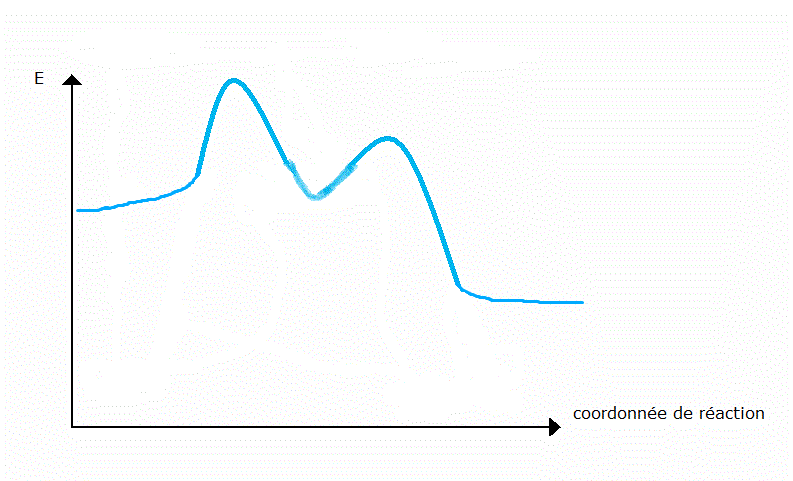
\includegraphics[scale=0.4]{E_act.png}
	\end{figure}
	
\begin{solution}

\begin{enumerate}
	\item \begin{solfig}{C}{Cinétique chimique}
		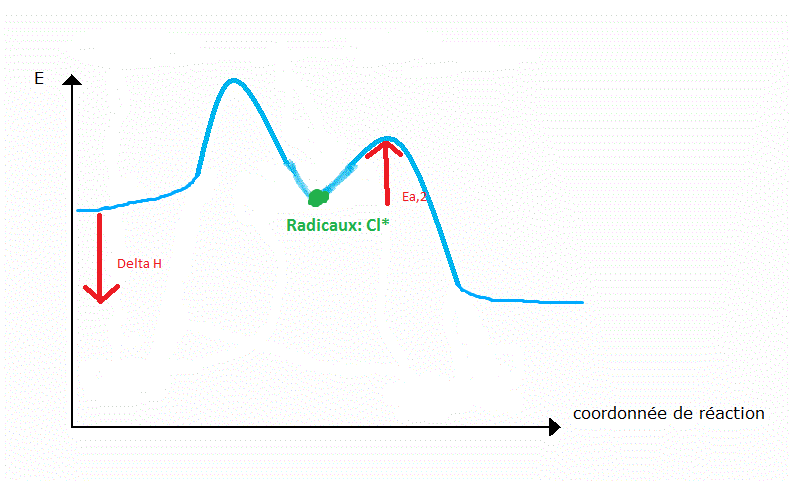
\includegraphics[scale=0.6]{E_act(sol).png}
		\end{solfig}
	\item La vitesse de formation des radicaux (composés créés lors de réactions élémentaires mais n'intervenant pas dans la réaction globale) 
	est égale à leur vitesse de disparition de telle sorte que ceux-ci n'apparaissent pas au niveau macroscopique.
	\item Puisque l'énergie d'activation de la réaction 1 est la plus élevée, celle-ci est la plus lente et détermine la vitesse de la réaction.
	Les vitesses des réactions sont 
	$$r_1=k_1[NO_2][Cl_2]\qquad r_1'=k_1'[ClNO_2][Cl]$$
	$$r_2=k_2[Cl][NO_2]\qquad r_2'=k_2'[ClNO_2]$$
	La vitesse globale vaut
	$$r=r_1=k_1[NO_2][Cl_2]$$
		
\end{enumerate}

	
\end{solution}

\section{Équilibre entre phases}

On considère deux volumes identiques contenant respectivement une mole et 3 moles d'un gaz parfait. Sachant que la température est de $300K$,
\begin{itemize}
    \item quelle la variation d'enthalpie libre due au mélange?
    \item quelle la variation d'enthalpie libre due au mélange si le mélange se fait à pression constante? Justifiez la différence par rapport au premier cas.
\end{itemize}

\begin{solution}

\begin{itemize}
    \item 
        On utilise
        $$\Delta_{\mbox{mél}} G=RT\sum\limits_{i} n_i\ln\frac{p_i}{p^i}=RT(\ln\frac{p_1}{p^i}+3\ln\frac{p_2}{p^i})$$
        On sait aussi que
        $$\mbox{ (pression partielle avant mélange)  }p^i=2p_i \mbox{ (pression partielle après mélange)}$$
        puisque le volume est doublé lors du mélange.
        $$\Rightarrow \Delta_{\mbox{mél}} G=RT(\ln(0,5)+3\ln(0,5))=-6915,8\;J$$
    \item 
        Pour un mélange isobare ($p^i=p$), on obtient:
        $$\Delta_{\mbox{mél}} G=RT\sum\limits_{i} n_i\ln\frac{p_i}{p}=RT\sum\limits_{i} n_i\ln (x_i)=RT(\ln(x_1)+3\ln(x_2))$$
        $$=RT(\ln(0,25)+3\ln(0,75))=-5610,6\:J$$
        La variation d'enthalpie libre pour un mélange isobare est supérieure, le mélange est donc moins stable. C'est parce que mélange absorbe de la chaleur pour augmenter la température et donc maintenir sa pression constante.
            
\end{itemize}

\end{solution}

\section{QCM}

\begin{enumerate}
    \item Quelle est l'activité d'une solution de $NaOH$ ($0,5M$) dont la pression de vapeur vaut 749 torr à 100$^\circ C$? (760 torr=1 atm)
    \begin{itemize}
        \item $0,986 \:atm$
        \item $0,986$
        \item $0,5$
        \item $0,5\:atm$
        \item Pas assez d'infos pour pouvoir répondre
    \end{itemize}

    \item Afin de mesure le débit d'eau dans une conduite de \SI{100}{\milli\meter} de diamètre, on réalise localement une contraction régulière avec un rapport de diamètre de 4. La chute de pression locale est mesurée à \SI{2000}{\pascal}. Quel est approximativement le débit dans la conduite ?
    
    \item Un composé a son point triple à 300$^\circ C$ et 1,2 bar. Quelle transformation parmi les suivantes le composé subit-il lorsqu'il passe de 290$^\circ C$ à 310$^\circ C$ sous une pression ambiante?
    \begin{itemize}
        \item Solide $\to$ vapeur
        \item Solide $\to$ liquide
        \item Vapeur $\to$ liquide
        \item Solide $\to$ gaz
        \item Liquide $\to$ vapeur
    \end{itemize}
    
    \item Que vaut le potentiel électrochimique d'une cellule plongée à température ambiante dans une solution d'ions $Ni^{2+}$ ($0,2M$) et $Zn^{2+}$ ($0,1M$)? 
    
    $E_{Zn^{2+}/Zn}^\circ=0,76V$ et $E_{Ni^{2+}/Ni}^\circ=0,14V$
    
    \item Dans un système ouvert, un gaz (assimilé à de l'air, gaz parfait diatomique) subit une transformation dans une machine thermique adiabatique réversible et passe d'une pression de 1 bar à une pression de 2,5 bar. La température initiale vaut 300K et le débit de fluide est de 50 g/s. Que vaut le travail moteur (en J/s) à fournir par la machine si son rendement est de 0,9? On néglige tout terme lié à l'énergie cinétique et le terme lié aux frottements est pris en compte dans le rendement.
    
    \item Dans une électrode standard à hydrogène, que vaut le potentiel électrochimique (à 298 K) dans une solution à pH 4,75?
    
    \item Quelle expression parmi les suivantes n'est \textbf{pas} correcte
	
    \begin{align*}
	    & V = -(\fpart{H}{p})_S 
    	& (\fpart{H}{S})_p = T &
    	&(\fpart{T}{V})_S = (\fpart{p}{S})_V&
    	&(\fpart{T}{p})_S = (\fpart{V}{S})_p
    \end{align*}
    
    \item On a une réaction ($A\Rightarrow B$) d'ordre global 1 ou 2 pour laquelle le temps de conversion de 10\% des réactifs dépend de la concentration initiale en réactifs. Laquelle de ces propositions est correcte?
    \begin{itemize}
        \item Le graphe de $[A]$ en fonction du temps est une droite.
        \item Le graphe de $1/[A]$ en fonction du temps est une droite.
        \item Le graphe de $\ln[A]$ en fonction du temps est une droite.
        \item Le graphe de $1/[A]$ en fonction de $1/t$ est une droite.
        \item Le graphe de $\ln[A]$ en fonction de $1/t$ est une droite.
    \end{itemize}
    
    \item Que vaut la capacité calorifique à pression constante d'un gaz parfait diatomique?
    
    \item Une machine frigorifique travaille selon un cycle de Carnot inversé entre une température extérieur de $\SI{25}{\celsius}$ et une température intérieure de $\SI{-10}{\celsius}$. Quel est le coefficient de performance de cette machine?

\end{enumerate}

\begin{solution}

\begin{enumerate}
    \item $a_i=p_i/p_i^\circ=\frac{0,986\:atm}{1 \:atm}=0,986$
    \item 1 [kg/s]
   $$ c_1^2=\bigg(\frac{A_2}{A_1}\bigg)^2c^2_2=\bigg(\frac{R_2}{R_1}\bigg)^4c^2_2$$
   $$ \Delta p=-\frac{\rho}{2} \Delta c^2=-\frac{\rho}{2}\bigg(1-\Big(\frac{R_2}{R_1}\Big)^4\bigg)c^2_2 \Rightarrow c_2^2=\frac{-2\Delta p}{\rho \bigg(1-\Big(\frac{R_2}{R_1}\Big)^4\bigg)}=4,0159$$
   $$ \dot V=\pi R_2^2c_2=\pi*(0,05/4)^2*\sqrt{4,0159}=10^{-3}\:[m^3/s] $$
        
    \item Solide $\to$ vapeur
        \begin{solfig}{P}{Cinétique chimique}
		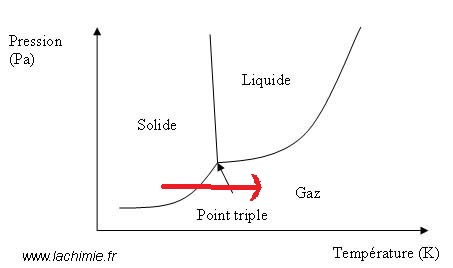
\includegraphics[scale=0.4]{diagramme-phase-eau.jpg}
	    \end{solfig}
    \item Le composé avec le potentiel le plus grand réagit à la cathode.
    \begin{itemize}
        \item Cathode: $Zn^{2+}+2e^-\Rightarrow Zn$
        \item Anode: $Ni^{2+}+2e^-\Rightarrow Ni$
    \end{itemize}
    $$E_{cell}=0,76-0,14+\frac{RT}{2F}\ln\frac{[Zn^{2+}]}{[Ni^{2+}]}=0,62+\frac{8,3145*298}{2*96485}\ln\frac{0,1}{0,2}=0,611\:V$$
    \item En système ouvert, $w_m=\Delta h=c_p\Delta T$
        Pour une transformation adiabatique:
       $$ T_2=T_1\bigg(\frac{p_1}{p_2}\bigg)^{\frac{1-\gamma}{\gamma}}=389,78K$$
       On trouve ainsi
       $$w_m=\frac{7}{2}*8,3145*(389,78-300)=2612,6\:J/mol$$
       $$W_{m,th}=\dot m\:w_m/M_m=\frac{2612,6}{28,96*10^{-3}}*0,05=4510,8\:J/s$$
       $$\Rightarrow W_{m,\mbox{réel}}=W_{m,th}/\eta=5012\:J/s$$
        
    \item 
        $$[H^+]=10^{-pH}=1,778*10^{-5}M$$
        Dans la réaction $2H^++2e^-\Rightarrow H_2$, le potentiel s'écrit
        $$E_{H^+/H}=E_{H^+/H}^\circ+\frac{RT}{2F}\ln ([H^+]^2)=0+\frac{8,3145*298}{96485}\ln 1,778*10^{-5}=-0,28V$$
    \item $-(\fpart{H}{p})_S = V$
				$$\mbox{d}H=\mbox{d}(U+pV)=\mbox{d}(Q+W+pV)=\mbox{d}Q-p\mbox{d}V+p\mbox{d}V+V\mbox{d}p=T\mbox{d}S+V\mbox{d}p$$
				Mais on sait aussi que
				$$\mbox{d}H(p,S)=(\fpart{H}{p})_S \mbox{d}p +(\fpart{H}{S})_p \mbox{d}S$$
				On a donc par identification:
				$$(\fpart{H}{p})_S = V \qquad (\fpart{H}{S})_p = T$$
    \item La réaction est d'ordre 2 puisque le temps de conversion de 10$\%$ de $A$ vaut $\ln(10)/k$ pour une réaction d'ordre 1.
    
    Le graphe de $1/[A]$ en fonction du temps est donc une droite.
    \item $c_p=\frac{7}{2}R$
    \item COP=$\frac{1}{\frac{T_{HOT}}{T_{COOL}}-1}=7,5$

\end{enumerate}

\end{solution}

\end{document}



